\documentclass{article}

\usepackage{arxiv}

\usepackage[utf8]{inputenc} % allow utf-8 input
\usepackage[T1]{fontenc}    % use 8-bit T1 fonts
\usepackage{hyperref}       % hyperlinks
\usepackage{url}            % simple URL typesetting
\usepackage{booktabs}       % professional-quality tables
\usepackage{amsfonts}       % blackboard math symbols
\usepackage{nicefrac}       % compact symbols for 1/2, etc.
\usepackage{microtype}      % microtypography
\usepackage{cleveref}       % smart cross-referencing
\usepackage{lipsum}         % Can be removed after putting your text content
\usepackage{graphicx}
\usepackage{natbib}
\usepackage{doi}
\usepackage{listings}

% Define custom colors for code highlighting
\usepackage{xcolor}
\definecolor{codegreen}{RGB}{50,205,50}
\definecolor{codegray}{RGB}{128,128,128}
\definecolor{codepurple}{RGB}{255,0,255}
\definecolor{backcolour}{RGB}{240,240,240}

% Define custom font for code listing
\usepackage{inconsolata}
\lstset{basicstyle=\ttfamily\footnotesize,breaklines=true}

% Set up the listings environment
\lstset{
    language=Python,
    commentstyle=\color{codegreen},
    keywordstyle=\color{blue},
    stringstyle=\color{codepurple},
    numberstyle=\tiny\color{codegray},
    basicstyle=\ttfamily\footnotesize,
    breakatwhitespace=false,
    breaklines=true,
    captionpos=b,
    keepspaces=true,
    numbers=left,
    numbersep=5pt,
    showspaces=false,
    showstringspaces=false,
    showtabs=false,
    tabsize=2,
    frame=single,
    backgroundcolor=\color{backcolour},
}

\title{High-Frequency Trading and Platform for Financial Research}

% Here you can change the date presented in the paper title
%\date{September 9, 1985}
% Or remove it
%\date{}

\author{ 
	% \href{https://orcid.org/0000-0000-0000-0000}{
\includegraphics[scale=0.06]{orcid.pdf}\hspace{1mm}David S.~Hippocampus}\thanks{Use footnote for providing further
	% 	information about author (webpage, alternative
	% 	address)---\emph{not} for acknowledging funding agencies.} 
	Shiwen An \\
	Department of Particles and Nuclear Studies\\
	The Graduate University for Advanced Studies, SOKENDAI\\
	Oho 1-1, Tsukuba, Japan \\
	\texttt{sweynan@icloud.com} \\
	%% examples of more authors
	% \And
	% \href{https://orcid.org/0000-0000-0000-0000}{
\includegraphics[scale=0.06]{orcid.pdf}\hspace{1mm}Elias D.~Striatum} \\
	% Department of Electrical Engineering\\
	% Mount-Sheikh University\\
	% Santa Narimana, Levand \\
	% \texttt{stariate@ee.mount-sheikh.edu} \\
	%% \AND
	%% Coauthor \\
	%% Affiliation \\
	%% Address \\
	%% \texttt{email} \\
	%% \And
	%% Coauthor \\
	%% Affiliation \\
	%% Address \\
	%% \texttt{email} \\
	%% \And
	%% Coauthor \\
	%% Affiliation \\
	%% Address \\
	%% \texttt{email} \\
}

% Uncomment to override  the `A preprint' in the header
%\renewcommand{\headeright}{Technical Report}
%\renewcommand{\undertitle}{Technical Report}
\renewcommand{\shorttitle}{\textit{arXiv} Template}

%%% Add PDF metadata to help others organize their library
%%% Once the PDF is generated, you can check the metadata with
%%% $ pdfinfo template.pdf
% \hypersetup{
% pdftitle={A template for the arxiv style},
% pdfsubject={q-bio.NC, q-bio.QM},
% pdfauthor={David S.~Hippocampus, Elias D.~Striatum},
% pdfkeywords={First keyword, Second keyword, More},
% }

\begin{document}
\maketitle

\begin{abstract}
	High frequency trading (HFT) is a form of algorithmic trading that involves using powerful computer programs and high-speed networks to execute a large number of trades in fractions of a second. The goal of HFT is to profit from very small price movements in financial markets, typically by buying and selling large volumes of securities, such as stocks, futures contracts, or currencies, in a matter of milliseconds.
\end{abstract}


% keywords can be removed
\keywords{ High-Frequency Trading \and Financial Platform Data \and Algorithms}


\section{Introduction}
HFT relies on sophisticated algorithms and advanced technologies, including ultra-low latency data feeds, high-speed trading platforms, and co-location services, which enable traders to access market data and execute trades faster than their competitors. HFT firms use complex mathematical models to identify and exploit market inefficiencies, such as price discrepancies between different exchanges or variations in supply and demand.

HFT has become increasingly popular in recent years, as technological advancements and regulatory changes have made it easier and cheaper for firms to engage in this type of trading. However, HFT has also been controversial, with critics arguing that it can lead to market instability, create unfair advantages for certain traders, and contribute to increased volatility and systemic risk.

There are many different algorithms used in high frequency trading, and the specific ones used by a particular firm may vary depending on their trading strategies and market conditions. However, some of the most commonly used algorithms in HFT include \textbf{Market Making, Statistical Arbitrage, Trend Following, and etc. } which will be introduced in the next section. 

\section{Common Strategies}

\begin{itemize}
	\item Market Making: This algorithm is used to provide liquidity to the market by continuously quoting bid and ask prices for a security, and buying and selling at those prices as orders come in.
	
	\item Statistical Arbitrage: This algorithm involves identifying mispricings in related securities and taking advantage of them by simultaneously buying and selling those securities.
	\item Trend Following: This algorithm uses technical analysis to identify trends in a security's price and then buys or sells based on whether the trend is up or down.
	\item News-Based Trading: This algorithm uses natural language processing techniques to analyze news and social media feeds for market-moving information, and then executes trades based on the results.
	\item Scalping: This algorithm involves quickly buying and selling securities to capture small price movements and earn profits on a large number of trades.
	\item Mean Reversion: This algorithm is based on the idea that prices tend to revert to their mean over time, and involves buying or selling a security when its price deviates significantly from its historical average. \cite{brogaard2014high}
\end{itemize}

% \subsection{Headings: second level}
% \begin{equation}
% 	\xi _{ij}(t)=P(x_{t}=i,x_{t+1}=j|y,v,w;\theta)= {\frac {\alpha _{i}(t)a^{w_t}_{ij}\beta _{j}(t+1)b^{v_{t+1}}_{j}(y_{t+1})}{\sum _{i=1}^{N} \sum _{j=1}^{N} \alpha _{i}(t)a^{w_t}_{ij}\beta _{j}(t+1)b^{v_{t+1}}_{j}(y_{t+1})}}
% \end{equation}

% \subsubsection{Headings: third level}
% \paragraph{Paragraph}


\section{Data and Financial Research Platform}
The choice of data sources will depend on the specific research question and the type of trading strategy being developed. High-frequency trading research often requires access to large amounts of high-quality data and the ability to process and analyze this data quickly and efficiently.
Here I give some brief summary for what kind of data source and simulation is possible for HFT research. 
\subsection{Brownian Motion}
\label{sec:others}
The most in-depth significantly cited paper is from here \cite{campbell1997econometric}. 
In some common event, Geometric Brownian Motion is applied.
\begin{equation}
dS_t = \mu S_t dt + \sigma S_t dW_t
\end{equation}
The equation for geometric Brownian motion is used to 
generate simulated financial data that exhibits similar 
statistical properties to real financial data. 
The equation describes the stochastic evolution 
of the price of an asset over time, 
taking into account both the expected mean 
return and the random fluctuations in price due to volatility.

To generate simulated financial data, we use the equation to calculate the price of an asset at each time step. We begin with an initial price, $S_0$, and simulate the price at the next time step using the equation:
\begin{equation}
	S_{t} = S_{0} e^{(\mu - \frac{\sigma^2}{2})t + \sigma \sqrt{t}Z}
\end{equation}
where $\Delta t$ is the time step, $\mu$ is the drift rate, $\sigma$ is the volatility, and $Z_1$ is a standard normal random variable.

We can continue this process to generate prices at each subsequent time step, using the current price and a new random variable at each step:
\begin{equation}
	S_{t+1} = S_{t} e^{(\mu - \frac{\sigma^2}{2})\Delta t + \sigma \sqrt{\Delta t}Z_{t+1}}
\end{equation}
By simulating many paths using this equation, we can generate a set of financial data that exhibits similar statistical properties to real financial data, including fat tails, volatility clustering, and autocorrelation. This can be useful for testing and developing trading strategies, risk models, and other financial applications.

\begin{scriptsize}
\begin{lstlisting}[language=Python]
	import numpy as np
	def generate_gbm(mu, sigma, S0, T, dt):
		N = int(T / dt)
		prices = np.zeros(N+1)
		prices[0] = S0
		Z = np.random.standard_normal(N)
		for i in range(1, N+1):
			prices[i] = prices[i-1] * np.exp((mu - 0.5*sigma**2)*dt + sigma*np.sqrt(dt)*Z[i-1])
	
		return prices
\end{lstlisting}
\end{scriptsize}
\begin{figure}
	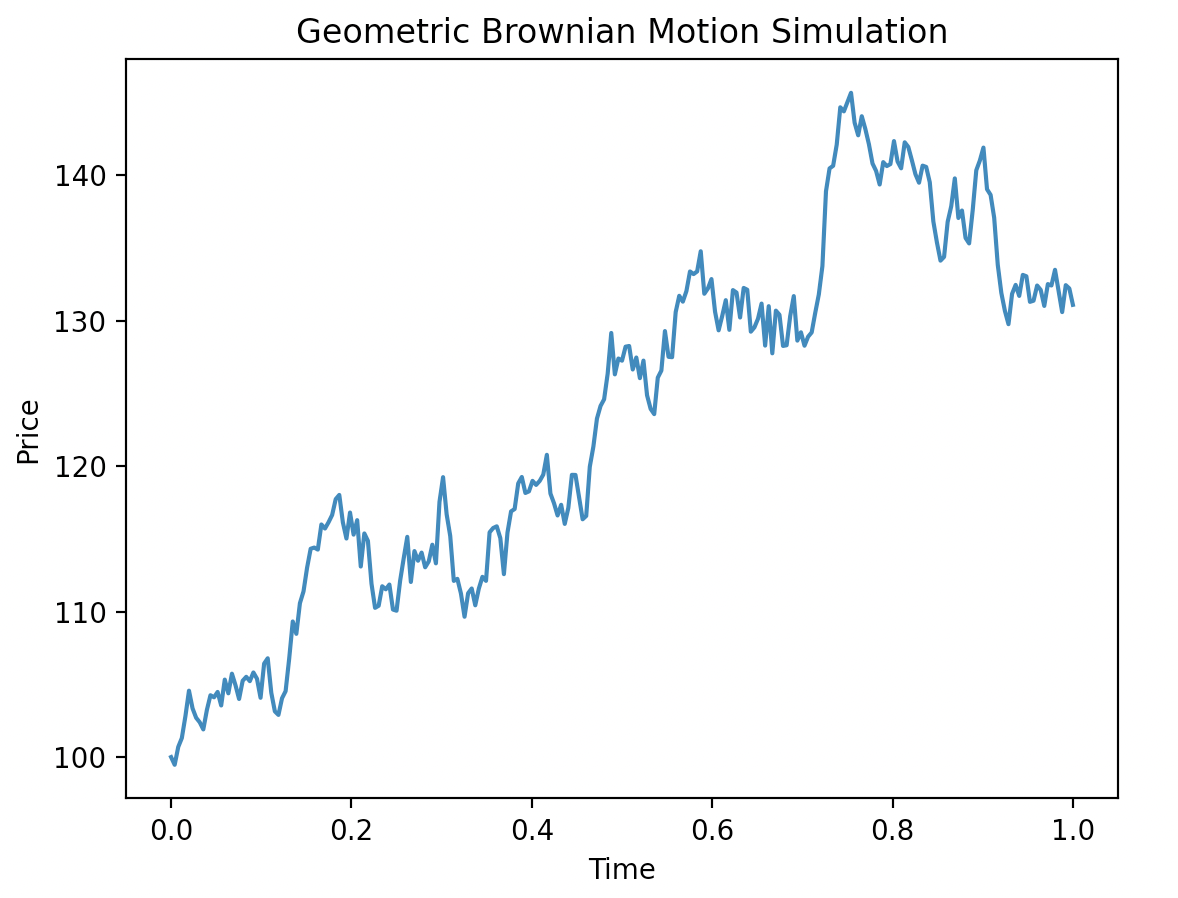
\includegraphics[width=0.32\linewidth]{GBM1.png}
	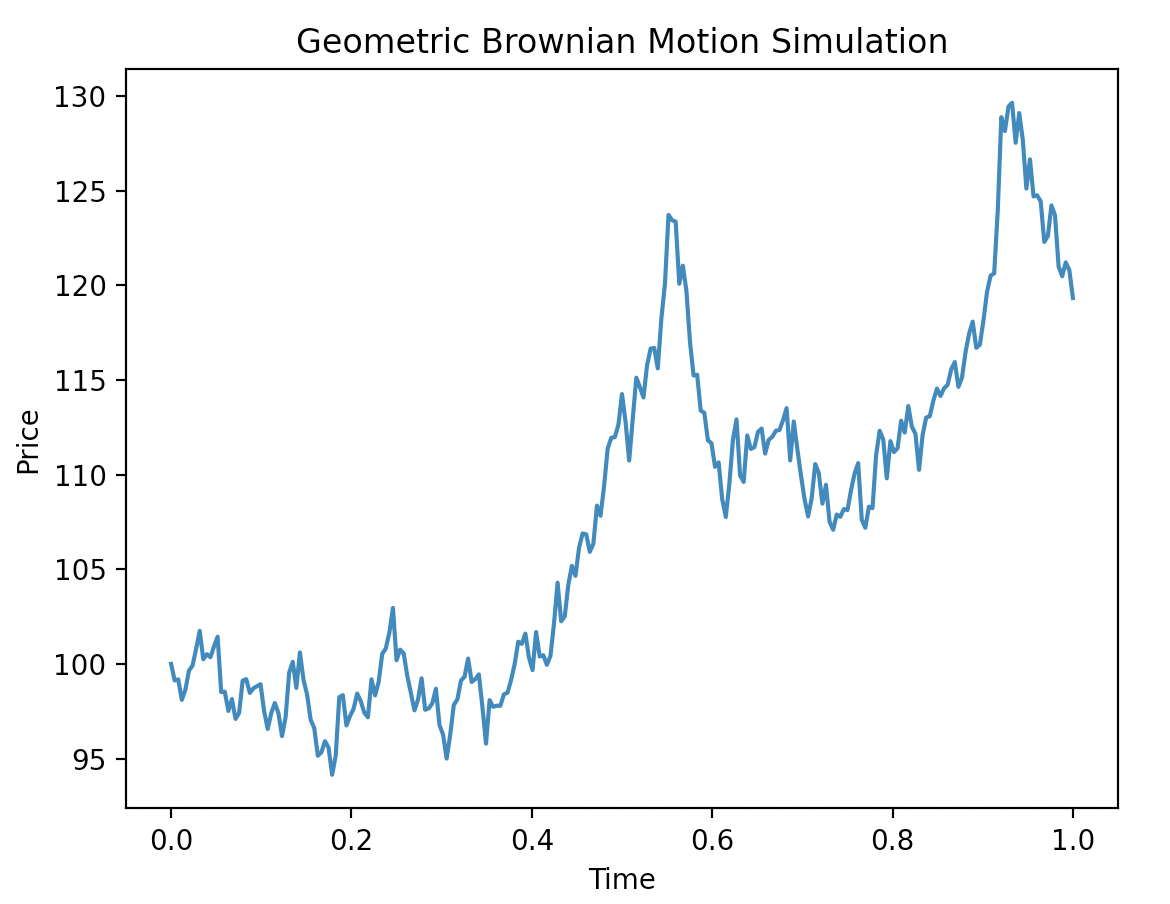
\includegraphics[width=0.32\linewidth]{GBM2.png}
	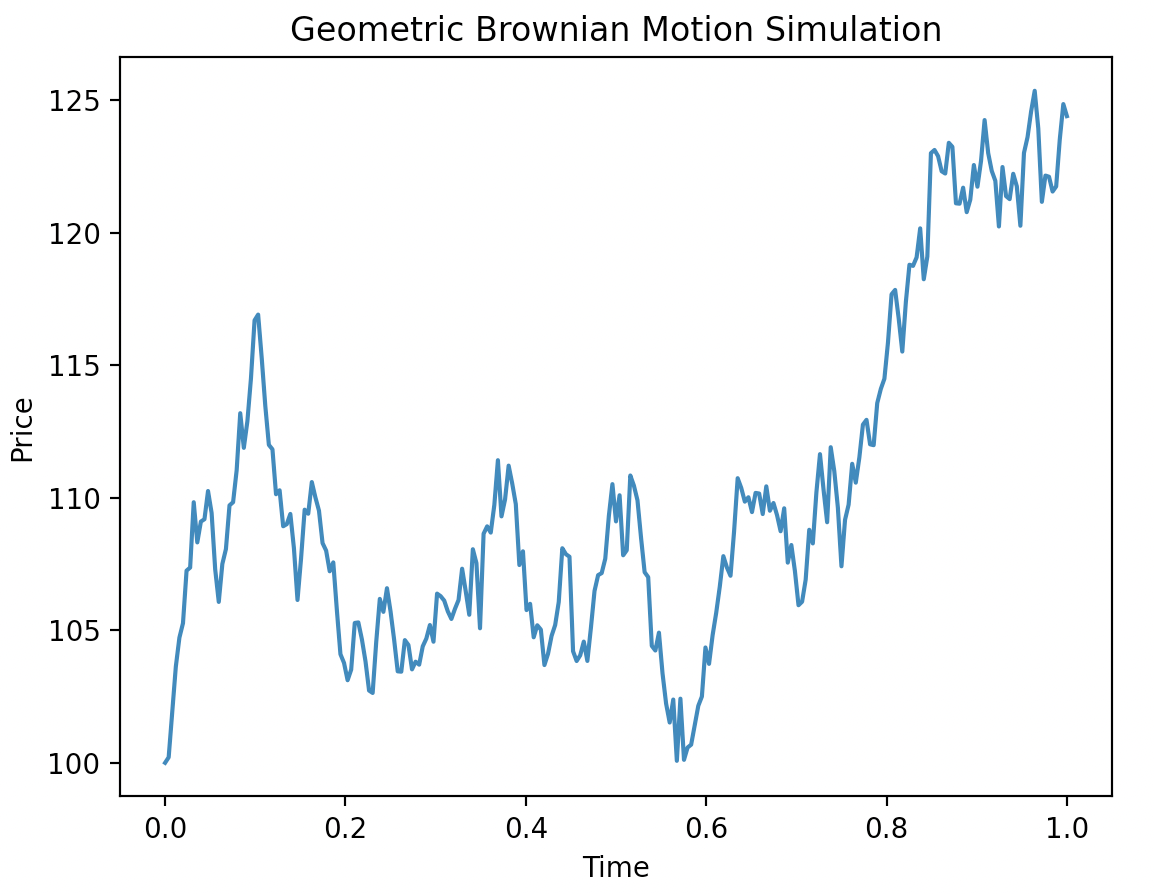
\includegraphics[width=0.32\linewidth]{GBM3.png}
	\caption{Geometric Brownian Motion Generated Diagram. Frequently used for 
	random in the Financial Research. }
\end{figure}
However, simulated data does not always work on the the real market. The data here could 
just be used for primitive research. 
\subsection{Market Data}

For research on abnormal spike on the market, NYSE Trade and Quote database \href{https://www.nyse.com/market-data/historical/daily-taq}{link} is a popular option 
\cite{campbell1997econometric}.  There is also case study using E-mini S\&P 500 Market Value, which drop in short 
period of time and caused a 'flash crash', where this part of data is part of historical data. \cite{kirilenko2011microstructure}.
Some financial firms employed HFT strategies usually collect their own market data and 
other papers also use Deutsche Boerse DAX index stocks \cite{brogaard2014high}, and one section in this research 
highlight the dataset when considering different task. CRSP data is considered for daily data not included in the HFT dataset, 
Compustat data are used to incorporate stock characteristics in to the analysis, and Trade and Quote (TAQ) data are used to incorporate additional intraday information
\cite{brogaard2014high}. The CBOE S\&P 500 Volatility Index (VIX) to capture market-wide volatility \cite{brogaard2014high}.


\subsection{Pros and Cons with Market Data}
Market data is one of the most commonly used data sources in high-frequency trading (HFT) research, and it has several advantages and disadvantages that should be considered when conducting research in this area.

Pros of using Market Data for research in HFT:
\begin{enumerate}
	\item High-quality data: Market data is generally of high quality and is available in real-time or historical form, allowing researchers to analyze market trends and identify trading opportunities.
	\item Wide availability: Market data is widely available from a variety of sources, including exchanges and data providers. This makes it easy for researchers to obtain and analyze the data they need.
	\item Relevance: Market data is directly related to trading activity and can provide valuable insights into market trends and investor sentiment.
	\item Accuracy: Market data is typically very accurate, as it is collected and maintained by highly regulated exchanges and data providers.
	\item Standardization: Market data is often standardized, which makes it easy to compare and analyze across different markets and asset classes.
\end{enumerate}
Cons of using Market Data for research in HFT:
\begin{enumerate}
	\item Expensive: Market data can be expensive to obtain, particularly if real-time data is required. This can be a barrier to entry for smaller research teams or individual traders.
	\item Latency: Market data can suffer from latency issues, particularly when real-time data is being used. This can impact the accuracy of trading strategies and make it difficult to compete with faster traders.
	\item Limited history: Market data is typically only available for a limited period of time, which can make it difficult to backtest trading strategies over longer timeframes.
	\item Noisy: Market data can be noisy and may contain irrelevant information, which can make it difficult to identify useful patterns or trends.
	\item Lack of transparency: Market data can lack transparency, particularly when it comes to dark pools and other off-exchange trading venues. This can make it difficult to obtain a complete picture of market activity.
\end{enumerate}
Market data is a valuable resource for high-frequency trading research, but it has some limitations that should be considered. 
Researchers should be aware of the potential biases 
and limitations of market data and use it in combination with other data sources to obtain a complete picture of market activity.

For both the strategy and the dataset, \cite{gomber2011high} provides better review for more details.
Here I just simply provide a summary for what HFT usually works. In my personal opinion, it is just another 
algorithm trading with higher processing speed on the market. 

\bibliographystyle{unsrtnat}
\bibliography{references}  %%% Uncomment this line and comment out the ``thebibliography'' section below to use the external .bib file (using bibtex) .


%%% Uncomment this section and comment out the \bibliography{references} line above to use inline references.
% \begin{thebibliography}{1}

% 	\bibitem{kour2014real}
% 	George Kour and Raid Saabne.
% 	\newblock Real-time segmentation of on-line handwritten arabic script.
% 	\newblock In {\em Frontiers in Handwriting Recognition (ICFHR), 2014 14th
% 			International Conference on}, pages 417--422. IEEE, 2014.

% 	\bibitem{kour2014fast}
% 	George Kour and Raid Saabne.
% 	\newblock Fast classification of handwritten on-line arabic characters.
% 	\newblock In {\em Soft Computing and Pattern Recognition (SoCPaR), 2014 6th
% 			International Conference of}, pages 312--318. IEEE, 2014.

% 	\bibitem{hadash2018estimate}
% 	Guy Hadash, Einat Kermany, Boaz Carmeli, Ofer Lavi, George Kour, and Alon
% 	Jacovi.
% 	\newblock Estimate and replace: A novel approach to integrating deep neural
% 	networks with existing applications.
% 	\newblock {\em arXiv preprint arXiv:1804.09028}, 2018.

% \end{thebibliography}


\end{document}
